%\title{Poster in Gothenburg}
%%%%%%%%%%%%%%%%%%%%%%%%%%%%%%%%%%%%%%%%%
% a0poster Landscape Poster
% LaTeX Template
% Version 1.0 (22/06/13)
%
% The a0poster class was created by:
% Gerlinde Kettl and Matthias Weiser (tex@kettl.de)
% 
% This template has been downloaded from:
% http://www.LaTeXTemplates.com
%
% License:
% CC BY-NC-SA 3.0 (http://creativecommons.org/licenses/by-nc-sa/3.0/)
%
%%%%%%%%%%%%%%%%%%%%%%%%%%%%%%%%%%%%%%%%%

%----------------------------------------------------------------------------------------
%	PACKAGES AND OTHER DOCUMENT CONFIGURATIONS
%----------------------------------------------------------------------------------------

\documentclass[a0b,landscape]{a0poster}

\usepackage{multicol} % This is so we can have multiple columns of text side-by-side
\columnsep=100pt % This is the amount of white space between the columns in the poster
\columnseprule=3pt % This is the thickness of the black line between the columns in the poster

\usepackage[svgnames]{xcolor} % Specify colors by their 'svgnames', for a full list of all colors available see here: http://www.latextemplates.com/svgnames-colors

\usepackage{times} % Use the times font
%\usepackage{palatino} % Uncomment to use the Palatino font

\usepackage{graphicx} % Required for including images
\graphicspath{{figures/}} % Location of the graphics files
\usepackage{booktabs} % Top and bottom rules for table
\usepackage[font=small,labelfont=bf]{caption} % Required for specifying captions to tables and figures
\usepackage{amsfonts, amsmath, amsthm, amssymb} % For math fonts, symbols and environments
\usepackage{wrapfig} % Allows wrapping text around tables and figures

\usepackage[matrix,arrow,curve]{xy}

\newtheorem*{theorem}{Theorem}
\newtheorem*{lemma}{Lemma}
\newtheorem*{proposition}{Proposition}
\newtheorem*{remark}{Remark}
\newtheorem*{corollary}{Corollary}
\newtheorem*{definition}{Definition}
\newtheorem*{example}{Example}
\newtheorem*{scheme}{Scheme}

\begin{document}

%----------------------------------------------------------------------------------------
%	POSTER HEADER 
%----------------------------------------------------------------------------------------

% The header is divided into three boxes:
% The first is 55% wide and houses the title, subtitle, names and university/organization
% The second is 25% wide and houses contact information
% The third is 19% wide and houses a logo for your university/organization or a photo of you
% The widths of these boxes can be easily edited to accommodate your content as you see fit

\begin{minipage}[b]{0.85\linewidth}
\veryHuge \color{NavyBlue} \textbf{On the topological version of freedom for classical, operator and sequential operator spaces} \color{Black}\\ % Title
\Large\textbf{Sergei Shteiner \& Norbert Nemesh}\\ % Author(s)
\Large Moscow State University\\ % University/organization
\end{minipage}
%
%
\begin{minipage}[b]{0.15\linewidth}
\begin{center}
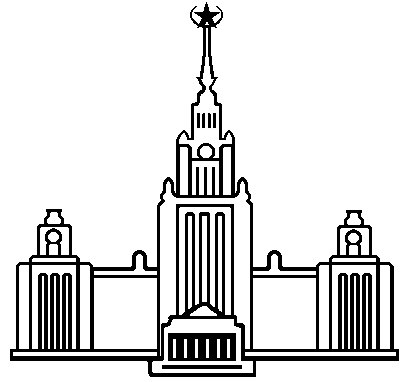
\includegraphics[width=10cm]{Eep8BvgUZEk.jpg} % Logo or a photo of you, adjust its dimensions here
\end{center}
\end{minipage}

%\vspace{1cm}  A bit of extra whitespace between the header and poster content

%----------------------------------------------------------------------------------------

\begin{multicols}{4} % This is how many columns your poster will be broken into, a poster with many figures may benefit from less columns whereas a text-heavy poster benefits from more

\small

\section*{Introduction}


Consider the category $A-mod$ of left normed modules over a fixed normed unital algebra $A$ and their bounded morphisms. A normed $A$-module $P$ is called \textit{topologically 
(metrically) projective} if for each open map (strict coisometry) $\tau : Y \to X$, where $X, Y \in A-mod$, and each bounded morphism $\varphi : P \to X$, there exists a 
lifting (a lifting with the same norm) $\psi$ of $\varphi$ across $\tau$, that is a morphism making the diagram
$$
\xymatrix{
& {Y} \ar[d]^{\tau}\\
{P} \ar@{-->}[ur]^{\psi} \ar[r]^{\varphi} &{X}}
$$
commutative. Similarly, a normed $A$-module $I$ is called \textit{topologically (metrically) injective} if for each bounded below map (isometry) $\tau : X \to Y$, where 
$X, Y \in A-mod$, and each bounded morphism $\varphi : X \to I$, there exists an extension (an extension with the same norm) $\psi$ of $\varphi$ across $\tau$, that
is a morphism making the diagram
$$
\xymatrix{
& {Y} \ar@{-->}[dl]_{\psi}\\
{I}  &{X} \ar[l]_{\varphi} \ar[u]_{\tau}
}
$$
commutative.

The topological projectivity was studied by Gottfried K\"{o}te in the context of Banach spaces and by Niels Gr{\o}nbaek in the context of normed spaces. The metric projectivity was recently introduced by Alexander Helemskii. The both types of projectivity and injectivity can be considered as particular cases of a certain general categorical scheme. Let $\mathcal{K}$ be an arbitrary category. A 
\textit{rig} of $\mathcal{K}$ is a faithful covariant functor $\square : \mathcal{K} \to \mathcal{L}$, where $\mathcal{L}$ is a category. A pair consisting of a category 
and its rig is called \textit{rigged category}. Fix, for a time, a rigged category, say $\left (\mathcal{K}, \square : \mathcal{K} \to \mathcal{L}\right )$. We call a 
morphism $\tau$ in $\mathcal{K}$ an \textit{admissible epimorphism (admissible monomorphism)} if the morphism $\square(\tau)$ is a retraction (coretraction) in $\mathcal{L}$. An 
object $P$ ($I$) in $\mathcal{K}$ is called projective (injective) with respect to the rig $\square$ if for every admissible epimorphism (monomorphism) $\tau$ the map
$\operatorname{Hom}_{\mathcal{K}}(P,\tau):\operatorname{Hom}_{\mathcal{K}}(P,Y)\to\operatorname{Hom}_{\mathcal{K}}(P,X)$ 
($\operatorname{Hom}_{\mathcal{K}}(\tau,I):\operatorname{Hom}_{\mathcal{K}}(Y,I)\to\operatorname{Hom}_{\mathcal{K}}(X,I)$) is surjective. Later on we will give the definitions of 
rigs describing metric and topological projectivity and injectivity.

Now we define a free object for the rig. Let $M$ be an object in $\mathcal{L}$. An object $F$ in $\mathcal{K}$ is called \textit{$\square$-free ($\square$-cofree)}
object with the \text{base} $M$ if there exists an isomorphism of functors $\operatorname{Hom}_{\mathcal{K}}(F,-)\cong\operatorname{Hom}_{\mathcal{L}}(M,\square(-))$
($\operatorname{Hom}_{\mathcal{K}}(-,F)\cong\operatorname{Hom}_{\mathcal{L}}(\square(-),M)$). A rigged category is called \textit{freedom(cofreedom)-loving} if 
every object in $\mathcal{L}$ is a base of a free (cofree) object in $\mathcal{K}$. The following fact is the main reason to study these objects.

\begin{proposition}[Helemskii] If a rigged category $(\mathcal{K},\square)$ is $\square$-freedom(cofreedom)-loving, then all its
$\square$-projective (injective) objects are retracts of $\square$-free (cofree) objects.
\end{proposition}

It is worth to mention that in general for a given type of projectivity there are rigs giving different classes of free objects but the same capacity of projective objects.
Our nearest goal is to find $\square_{Met}$- and $\square_{Top}$-free and cofree objects for the case $A = \mathbb{C}$ and the categories of normed spaces, operator spaces,
sequential operator spaces and non-archimedian spaces.





%%%%%%%%%%%%%%%%%%%%%%%%%%%%%%%%%%%%%%%%%%%%%%%%%%%%%%%%%%%%%%%%%%%%%%%%%%%%%%%%%%%%%%%%%%%%%%%%%%%%%%%%%%%%%%%%%%%%%%%%%%%%%%%%%%%%%%%%%%%%%%%%%%%%%%%%%%%%%%%%%%%%%%%%%%%%%%%%%%%%%
%	Normed spaces
%%%%%%%%%%%%%%%%%%%%%%%%%%%%%%%%%%%%%%%%%%%%%%%%%%%%%%%%%%%%%%%%%%%%%%%%%%%%%%%%%%%%%%%%%%%%%%%%%%%%%%%%%%%%%%%%%%%%%%%%%%%%%%%%%%%%%%%%%%%%%%%%%%%%%%%%%%%%%%%%%%%%%%%%%%%%%%%%%%%%%





\section*{Normed spaces}

To put the metric projectivity in the general scheme, consider the functor
$$
\square_{Met}:Nor_1\to Set: X\mapsto Ball_X\quad \varphi\mapsto \varphi|_{Ball_X}^{Ball_Y}.
$$
It is almost immediate that in our case $\square_{Met}$-admissible epimorphisms are exactly strictly coisometric morphisms, and $\square_{Met}$-projective objects are exactly
metrically projective modules.


Let us now define the topological projectivity in this scheme. A \textit{semilinear} space over a field $K$ is a set $V$ together with a binary operation
$\cdot:K\times V\to V$ that satisfies the three axioms listed below:

1) for all $a,b\in K$ and $v\in V$ holds $a\cdot (b\cdot v) = ab\cdot v,$

2) for all $v\in V$ we have $1_K\cdot v=v,$

3) there exists $\mathbf{0} \in V$, such that $0_K\cdot v = \mathbf{0}$ for all $v \in V$.

A map $\varphi : V \to W$  between two semilinear spaces is said to be a \textit{semilinear} map if for each vector $v \in V$ and each scalar $\alpha\in K$,
the following condition is satisfied:  $\varphi(\alpha \cdot v) = \alpha \cdot \varphi(v)$.

A norm on a semilinear space $V$ over a valued field $K$ is a function $ \Vert  \cdot  \Vert  : V \to \mathbb{R}_{+}$, such that

1) $ \Vert  v  \Vert  = 0$ if and only if $v = \mathbf{0}$;

2) $ \Vert  \alpha \cdot v  \Vert  = | \alpha |  \Vert  v  \Vert $ for all $\alpha \in K$, and $v \in V$.

A normed semilinear space is a pair $(V,  \Vert  \cdot  \Vert  ),$ where $V$ is a semilinear space and $  \Vert  \cdot  \Vert  $ is a norm on $V$. By $Nor_0^K$ we denote the 
category of normed semilinear spaces over $K$ and bounded semilinear maps.  Let $\Lambda$ be a set and $K_{\lambda}=K$ for each $\lambda \in \Lambda$. One can show that any semilinear space is isomorphic in $Nor_0^K$ to the wedge sum 
$\bigvee\{K_{\lambda}: \lambda \in\Lambda\}$ of copies of pointed spaces $(K,0_K)$ for a certain set $\Lambda$.

Let now $K := \mathbb{C}$, then consider the functor
$$
\square_{Top}:Nor\to Nor_0: X\mapsto X\quad \varphi\mapsto \varphi
$$
which forgets about addition. One can check that in this case $\square_{Top}$-admissible epimorphisms
are exactly open morphisms, and $\square_{Top}$-projective objects are exactly topologically projective modules.

We will use the following observation.

\begin{proposition}[Helemskii] Suppose that $\mathcal{K}$ admits coproducts, $\mathcal{L}$ is just $Set$, and there
exists a free module, say $F$, with a one-point base. Then our rigged category is freedom-loving. Moreover, if $\Lambda$ is an arbitrary set, then the coproduct of the family
of copies of $F$, indexed by points of $\Lambda$, is the free object with the base $\Lambda$.
\end{proposition}

Metrically or topologically free objects with a one-point base are obviously one dimensional spaces, and coproducts in $Nor_1$ are their $l_1^0$-sums.
Thus metrically free objects are exactly $l_1^0(\Lambda)$ spaces and rigged category $(Nor_1, \square_{Met})$ is freedom-loving. For the topological freedom in general there 
is no coproducts in $Nor$, but the following proposition saves the day.

\begin{proposition} Let $E$ be a metrically free normed space with a base $\Lambda$. Then $E$ is topologically free with the base $\bigvee\{K_{\lambda} : \lambda \in\Lambda\}$. Conversely, 
let $E$ be a topologically free normed space with the base $\bigvee\{K_{\lambda}: \lambda \in\Lambda\}$. Then it is topologically isomorphic to some metrically free normed space $E^{'}$ 
with the base $\Lambda$.
\end{proposition}

Thus we obtain that topologically free spaces are also $l_1^0(\Lambda)$ (but in the category $Nor$) and the rigged category $(Nor, \square_{Top})$ is freedom-loving. Of course 
there is an easy straightforward proof of this fact, but this approach seems to be more convenient in more complicated cases discussed below.

Similarly, one can show that admissible monomorphisms for functors
$$
\square_{Met}^d:Nor_1\to Set^o: X\mapsto Ball_{X^*},\quad\varphi\mapsto \varphi^*|_{Ball_{Y^*}}^{Ball_{X^*}}
$$
$$
\square_{Top}^d:Nor\to Nor_0^o: X\mapsto X^*,\quad\varphi\mapsto \varphi^*
$$
are exactly isometric and bounded below morphisms respectively. We obtain the description of free objects. Now it is easy to describe cofree ones using the following result.

\begin{proposition}[Helemskii] Assume we are given two rigged categories $(\mathcal{K}_1, \square_1: \mathcal{K}_1 \to \mathcal{L}_1)$,
$(\mathcal{K}_2, \square_2 : \mathcal{K}_2 \to \mathcal{L}_2)$, and two covariant functors $\Phi : \mathcal{K}_1 \to \mathcal{K}_2$,
$\Psi : \mathcal{L}_1 \to \mathcal{L}_2$ such that the diagram is
$$
\xymatrix{
{\mathcal{K}_1}\ar[d]_{\Phi}
\ar[rr]^{\square_1} && {\mathcal{L}_1}\ar[d]^{\Psi}\\
{\mathcal{K}_2}\ar[rr]^{\square_2} &&{\mathcal{L}_2}}
$$
commutative. Assume $\Phi$ and $\Psi$ have left adjoint functors $\Phi^*$ and $\Psi^*$ respectively, and
$F\in\mathcal{K}_2$ is a $\square_2$-free object with base $M\in\mathcal{L}_2$. Then $\Phi^*(F)\in\mathcal{K}_1$
is a $\square_1$-free object with base $\Psi^*(M)\in\mathcal{L}_1$. In particular if
$(\mathcal{K}_2,\square_2)$ is freedom-loving then so does $(\mathcal{K}_1,\square_1).$
\end{proposition}

One can check that the assumptions of this proposition hold for the pairs of functors $((\square_{Met}^d)^o,\square_{Met})$ and $((\square_{Top}^d)^o,\square_{Top})$ with
$\Phi$ as ${}^*$ functor and $\Psi$ as an identity functor. Hence metrically (topologically) cofree normed spaces are exactly $(\ell_1^0(\Lambda))^*=\ell_\infty(\Lambda)$ 
for some set $\Lambda$.

\begin{scheme}
All in all, the solution above consists of four basic steps:

1) We find a free object with a one-point base.

2) We notice that the category in question admits coproducts, so free objects are exactly the coproducts of copies of free objects with a one-point base.

3) We prove that all metrically free objects are topologically free.

4) We check that the conditions of the previous proposition hold, so metrically and topologically cofree objects are duals of free ones.
\end{scheme}

This scheme can be applied to the categories we are going to discuss right now --- operator spaces, sequential operator spaces and non-archimedean spaces.






%%%%%%%%%%%%%%%%%%%%%%%%%%%%%%%%%%%%%%%%%%%%%%%%%%%%%%%%%%%%%%%%%%%%%%%%%%%%%%%%%%%%%%%%%%%%%%%%%%%%%%%%%%%%%%%%%%%%%%%%%%%%%%%%%%%%%%%%%%%%%%%%%%%%%%%%%%%%%%%%%%%%%%%%%%%%%%%%%%%%%
%	Operator spaces
%%%%%%%%%%%%%%%%%%%%%%%%%%%%%%%%%%%%%%%%%%%%%%%%%%%%%%%%%%%%%%%%%%%%%%%%%%%%%%%%%%%%%%%%%%%%%%%%%%%%%%%%%%%%%%%%%%%%%%%%%%%%%%%%%%%%%%%%%%%%%%%%%%%%%%%%%%%%%%%%%%%%%%%%%%%%%%%%%%%%%




\section*{Operator spaces}

Operator spaces are well known but we feel obliged to recall necessary definitions. Let $E$ be a normed space, then for given $m,n\in\mathbb{N}$ by $M_{m,n}(E)$ we denote a complex linear space of $m\times n$ matrices with entries in $E$. By $\Vert\cdot\Vert_n$
we denote a norm on $M_{n,n}(E)$. We say that the pair $X=(E,\{\Vert\cdot\Vert_n:n\in\mathbb{N}\})$ defines the structure of \textit{operator space} on $E$ if 

1) for all $x\in M_{n,n}(E)$ and $\alpha\in M_{m,n}(\mathbb{C})$, $\beta\in M_{n,m}(\mathbb{C})$ we have
$
\Vert\alpha x\beta\Vert_m\leq\Vert\alpha\Vert\Vert x\Vert_n\Vert\beta\Vert,
$

2) for all $x\in M_{n,n}(E)$, $y\in M_{m,m}(E)$ we have
$
\Vert x\oplus y\Vert_{n+m}\leq\max(\Vert x\Vert_n,\Vert y\Vert_m),
$\\
where $m,n\in\mathbb{N}$. For example $\mathcal{B}(\mathbb{C}^k)$ can be endowed with this structure via the identification 
$M_{n,n}(\mathcal{B}(\mathbb{C}^k))=\mathcal{B}(\mathbb{C}^{nk})$.

For a given operator spaces $X$ and $Y$ and a linear operator $\varphi:X\to Y$ we define its $n$-th \textit{amplification} as a linear operator
$\varphi^n:M_{n,n}(X)\to M_{n,n}(Y):x\mapsto (\varphi(x_{ij})_{i,j=1,n})$. A linear operator $\varphi$ is called \textit{completely bounded} if its $cb$-norm
$\Vert \varphi\Vert_{cb}=\sup\{\Vert \varphi^n\Vert_{\mathcal{B}(M_n(X),M_n(Y)):n\in\mathbb{N}}\}$ is finite. 
The set of completely bounded operators between $X$ and $Y$ forms an operator space
$\mathcal{CB}(X,Y)$ with the sequence of norms given by the identification $M_{n,n}(\mathcal{CB}(X,Y))=\mathcal{CB}(X,M_{n,n}(Y))$.
Therefore in the operator space theory we have the analogue of
continuous dual space defined by $X^\triangle=\mathcal{CB}(X,\mathbb{C})$. In this case we can endow the space of nuclear operators $\mathcal{N}(H,K)$ between two Hilbert 
spaces $H$, $K$ with an operator space structure via the natural inclusion $\mathcal{N}(H,K)\hookrightarrow \mathcal{B}(K,H)^\triangle$. Then one can show that
$\mathcal{B}(\mathbb{C}^n)^\triangle=\mathcal{N}(\mathbb{C}^n)$ and $\mathcal{N}(\mathbb{C}^n)^\triangle=\mathcal{B}(\mathbb{C}^n)$.

Thus we can define two categories --- $QNor$ and $QNor_1$. Their objects are operator spaces. Their morphisms are completely bounded and completely contractive linear 
operators respectively.

The category $QNor_1$ admits products and coproducts. Let $\{X_ \lambda : \lambda \in \Lambda\}$ be a family of objects in $QNor_1$, then their product is a normed space
$\bigoplus_\infty\{M_{1,1}(X_ \lambda ): \lambda \in \Lambda\}$ with a sequence of norms induced by the identification 
$M_{n,n}\left(\bigoplus{}_\infty\{X_ \lambda : \lambda  \in \Lambda\}\right)=\bigoplus{}_\infty\{M_{n,n}(X_ \lambda ): \lambda \in \Lambda\}$. 
The coproduct is a normed space $\bigoplus{}_1^0\{M_{1,1}(X_ \lambda ): \lambda \in \Lambda\}$ with a sequence of norms induced by the inclusion
$\bigoplus{}_1^0\{X_ \lambda : \lambda  \in \Lambda\}\hookrightarrow\left(\bigoplus{}_\infty\{X_ \lambda ^\triangle: \lambda \in \Lambda\}\right)^\triangle.$

Let us define two types of admissible morphisms to introduce metric and topological projectivity and injectivity. We say that a morphism of operator spaces $\varphi$
is called \textit{completely strictly coisometric (open map)} if all its amplifications are strictly coisometric (open maps with the same coercivity constant). Along the same lines 
we say that a morphism of operator spaces $\varphi$ is called \textit{completely isometric (bounded below)} if all its amplifications are isometric (bounded below with the same
constant). One can check that the following four faithful functors
$$
\begin{aligned}
&\square_{qMet} : QNor_1 \to Set :  X\mapsto\prod_{n \in \mathbb{N}} Ball_{M_{n,n}(X)}\quad
\varphi\mapsto \prod_{n\in\mathbb{N}} \varphi^{n}|_{Ball_{M_{n,n}(X)}}^{Ball_{M_{n,n}(Y)}},\\
&\square_{qTop} : QNor \to Nor_0:  X \mapsto \bigoplus_{ n \in \mathbb{N}}{}_\infty M_{n,n}(X) \quad
\varphi\mapsto\bigoplus_{n\in\mathbb{N}}{}_\infty \varphi^{n},\\
&\square_{qMet}^d : QNor_1 \to Set : X\mapsto\prod_{n \in \mathbb{N}} Ball_{M_{n,n}(X^\triangle)}\quad
\varphi\mapsto \prod_{n\in\mathbb{N}} (\varphi^\triangle)^{n}|_{Ball_{M_{n,n}(Y^\triangle)}}^{Ball_{M_{n,n}(X^\triangle)}},\\
&\square_{qTop}^d : QNor \to Nor_0^o: X \mapsto \bigoplus_{ n \in \mathbb{N}}{}_\infty M_{n,n}(X^\triangle) \quad
\varphi\mapsto\bigoplus_{n\in\mathbb{N}}{}_\infty(\varphi^\triangle)^{n}
\end{aligned}
$$
describe metric and topological projectivity and injectivity in the category of operator spaces. One can show that
$\mathcal{N}_{\infty} := \bigoplus_1^0 \{\mathcal{N}(\mathbb{C}^n): n \in \mathbb{N}\}$ is metrically free with a one-point base. Moreover, all metrically free operator spaces 
are topologically free. So using the general scheme we conclude that all metrically and topologically free objects are of the form 
$\bigoplus_1^0\{\mathcal{N}_\infty: \lambda \in \Lambda\}$. 
Finally, following the general scheme we obtain the description of metrically and topologically cofree objects. They are
$\bigoplus_\infty\{\mathcal{B}_\infty: \lambda \in \Lambda\}$, where
$\mathcal{B}_{\infty} := \bigoplus_\infty \{\mathcal{B}(\mathbb{C}^n): n \in \mathbb{N}\}$.





%%%%%%%%%%%%%%%%%%%%%%%%%%%%%%%%%%%%%%%%%%%%%%%%%%%%%%%%%%%%%%%%%%%%%%%%%%%%%%%%%%%%%%%%%%%%%%%%%%%%%%%%%%%%%%%%%%%%%%%%%%%%%%%%%%%%%%%%%%%%%%%%%%%%%%%%%%%%%%%%%%%%%%%%%%%%%%%%%%%%%
%	Sequential operator spaces
%%%%%%%%%%%%%%%%%%%%%%%%%%%%%%%%%%%%%%%%%%%%%%%%%%%%%%%%%%%%%%%%%%%%%%%%%%%%%%%%%%%%%%%%%%%%%%%%%%%%%%%%%%%%%%%%%%%%%%%%%%%%%%%%%%%%%%%%%%%%%%%%%%%%%%%%%%%%%%%%%%%%%%%%%%%%%%%%%%%%%




\section*{Sequential operator spaces}

Sequential operator spaces were introduced and studied by Anselm Lambert in his PhD thesis in 2002. Informally speaking these spaces are situated between classical Banach spaces and 
operator spaces. Let $E$ be a linear space, and for each $n\in\mathbb{N}$ we have a linear space $E^n:=\oplus_{k=1}^n E$ and a norm on $\Vert \cdot \Vert_{\widehat{n}}:E^n\to\mathbb{R}_+$.
We say that the pair $X = (E^n, \{\Vert \cdot \Vert_{\widehat{n}}:n\in\mathbb{N}\})$ defines the structure of \textit{sequential operator space} on $E$, if
the following conditions are satisfied:

1) for all $x \in E^{\widehat{n}}$, $\alpha \in M_{m, n}(\mathbb{C})$ holds
$
\Vert \alpha x \Vert_{\widehat{m}} \leq \Vert \alpha \Vert  \Vert x \Vert_{\widehat{n}},
$

2) for all $x \in E^n$, $y \in E^m$ holds
$
\left\Vert ( x, y ) \right\Vert^2_{\widehat{n + m}} \leq   \Vert x \Vert_{\widehat{n}}^2 + \Vert y \Vert_{\widehat{m}}^2,
$\\
where $m,n\in\mathbb{N}$. By $X^{\widehat{n}}$ we will denote the normed space $(E^n,\Vert \cdot \Vert_{\widehat{n}})$.

An obvious example of such structure is the one-dimensional complex linear space $l_2^n,$ which is just $\mathbb{C}$ with norms defined by the identification $\mathbb{C}^{\widehat{n}}=\mathbb{C}^n$. 
Next example is the $n$-dimensional complex linear space $t_2^n$ with a sequence of norms defined by the identification
$(t_2^n)^{\widehat{k}}=\mathcal{B}(\mathbb{C}^k,\mathbb{C}^n)$.

If $X$ and $Y$ are two sequential operator spaces and $\varphi : X \rightarrow Y$ is a linear operator, then for each $n\in\mathbb{N}$ its $n$-th \textit{amplification} is  
a linear operator $\varphi^{\widehat{n}} : X^{\widehat{n}} \to Y^{\widehat{n}}$ defined by $\varphi^{\widehat{n}}(x)=(\varphi(x_i))_{i=1,n}$. We say that $\varphi$ 
is \textit{sequentially bounded}, if $sb$-norm $\Vert \varphi \Vert_{sb} := \sup\{\Vert \varphi^{\widehat{n}}\Vert_{\mathcal{B}(X^{\widehat{n}},Y^{\widehat{n}})}:n\in\mathbb{N}\}$ 
is finite. The set of such operators forms a normed space $\mathcal{SB}(X,Y)$, which in turn can be endowed with a sequential operator space structure via the identification
$\mathcal{SB}(X,Y)^{\widehat{n}}=\mathcal{SB}(X,Y^{\widehat{n}})$. This allows us to introduce the notion of sequential dual of sequential operator space 
$X^\triangle:=\mathcal{SB}(X,\mathbb{C})$. One can show that $(t_2^n)^\triangle=l_2^n$ and $(l_2^n)^\triangle=t_2^n$.

Now we define two categories $SQNor$ and $SQNor_1$. Their objects are sequential operator spaces. Morphisms of the first category are sequentially bounded linear operators,
morphisms of the second category are sequentially bounded linear operators with $sb$-norm not greater than $1$.

Let $\{X_ \lambda : \lambda \in \Lambda\}$ be a family of objects in $SQNor_1$, then their product is a normed space
$\bigoplus_\infty\{X_ \lambda ^{\widehat{1}}: \lambda \in \Lambda\}$ with the sequence of norms induced by the identification 
$\left(\bigoplus{}_\infty\{X_ \lambda : \lambda  \in \Lambda\}\right)^{\widehat{n}} =\bigoplus{}_\infty\{X_ \lambda ^{\widehat{n}}: \lambda \in \Lambda\}$. 
The coproduct is a normed space $\bigoplus{}_1^0\{X_ \lambda ^{\widehat{1}}: \lambda \in \Lambda\}$ with a sequence of norms induces by the inclusion 
$\bigoplus{}_1^0\{X_ \lambda : \lambda  \in \Lambda\}\hookrightarrow \left(\bigoplus{}_\infty\{X_ \lambda ^\triangle: \lambda \in \Lambda\}\right)^\triangle.$

Let us define two types of admissible morphisms to introduce metric and topological projectivity and injectivity. We say that a morphism of sequential operator spaces $\varphi$
is called \textit{sequentially strictly coisometric (open map)} if all its amplifications are strictly coisometric (open maps with the same coercivity constant). Similarly
we say that a morphism of sequential operator spaces $\varphi$ is \textit{sequentially isometric (bounded below)} if all its amplifications are isometric 
(bounded below with the same constant). One can check that for the following four faithful functors
$$
\begin{aligned}
&\square_{sqMet} : SQNor_1 \to Set :  X\mapsto\prod_{n \in \mathbb{N}} Ball_{X^{\widehat{n}}}\quad
\varphi\mapsto \prod_{n\in\mathbb{N}} \varphi^{\widehat{n}}|_{Ball_{X^{\widehat{n}}}}^{Ball_{Y^{\widehat{n}}}},\\
&\square_{sqTop} : SQNor \to Nor_0:  X \mapsto \bigoplus_{n \in \mathbb{N}}{}_\infty X^{\widehat{n}}  \quad
\varphi\mapsto\bigoplus_{n\in\mathbb{N}}{}_\infty \varphi^{\widehat{n}},\\
&\square_{sqMet}^d : SQNor_1 \to Set : X\mapsto\prod_{n \in \mathbb{N}} Ball_{(X^\triangle)^{\widehat{n}}}\quad
\varphi\mapsto \prod_{n\in\mathbb{N}} (\varphi^\triangle)^{\widehat{n}}|_{Ball_{(Y^\triangle)^{\widehat{n}}}}^{Ball_{(X^\triangle)^{\widehat{n}}}},\\
&\square_{sqTop}^d : SQNor \to Nor_0^o: X \mapsto \bigoplus_{n \in \mathbb{N}}{}_\infty (X^\triangle)^{\widehat{n}} \quad
\varphi\mapsto\bigoplus_{n\in\mathbb{N}}{}_\infty (\varphi^\triangle)^{\widehat{n}}
\end{aligned}
$$
describe metric and topological projectivity and injectivity in the category of sequential operator spaces. One can show that
$t_2^{\infty} := \bigoplus_1^0 \{t_2^n: n \in \mathbb{N}\}$ is a metrically free with a one-point base and that every
metrically free object is topologically free, so using the general scheme we conclude that all metrically and topologically free objects are of the form
$\bigoplus_1^0\{t_2^\infty: \lambda \in \Lambda\}$. Follow the general scheme one can obtain the description of metrically and topologically cofree objects. They are
$\bigoplus_\infty\{l_2^\infty: \lambda \in \Lambda\}$, where $l_2^{\infty} := \bigoplus_\infty \{l_2^n: n \in \mathbb{N}\}$.






%%%%%%%%%%%%%%%%%%%%%%%%%%%%%%%%%%%%%%%%%%%%%%%%%%%%%%%%%%%%%%%%%%%%%%%%%%%%%%%%%%%%%%%%%%%%%%%%%%%%%%%%%%%%%%%%%%%%%%%%%%%%%%%%%%%%%%%%%%%%%%%%%%%%%%%%%%%%%%%%%%%%%%%%%%%%%%%%%%%%%
%	Non-archimedean spaces
%%%%%%%%%%%%%%%%%%%%%%%%%%%%%%%%%%%%%%%%%%%%%%%%%%%%%%%%%%%%%%%%%%%%%%%%%%%%%%%%%%%%%%%%%%%%%%%%%%%%%%%%%%%%%%%%%%%%%%%%%%%%%%%%%%%%%%%%%%%%%%%%%%%%%%%%%%%%%%%%%%%%%%%%%%%%%%%%%%%%%





\section*{Non-Archimedean spaces}

Let $K$ be a field, then \textit{non-Archimedean valuation} on $K$ is a function $|\cdot|:K\to \mathbb{R}_+$ such that for all $a,b\in K$ holds

1) $|ab|=|a||b|,$

2) $|a+b|\leq\max(|a|,|b|),$

3) $|a|=0$ if and only if $a=0.$

We additionally assume that the valuation is non-trivial, i.e. there exists $a\in K$ with $|a|\notin\{0,1\}$. Each valuation makes $K$ a metric space with a distance function 
$d(a,b)=|a-b|$. So $K$ is called a non-Archimedean field if it has a non-trivial valuation which makes $K$ a complete metric space. Most of results of classical functional 
analysis remains the same if we additionally require $K$ to be \textit{spherically complete}, i.e. any descending by inclusion chain of balls in $K$ has non-empty intersection.

Let $E$ be a linear space over $K$. The \textit{non-Archimedean norm} on $E$ is a function $\Vert\cdot\Vert:E\to\mathbb{R}_+$ such that

1) $\Vert a x\Vert=|a|\Vert x\Vert,$

2) $\Vert x+y\Vert\leq\max(\Vert x\Vert,\Vert y\Vert),$

3) $\Vert x\Vert=0$ if and only if $x=0$
\\
for all $x,y\in V$ and $a\in K$. A pair $(X,\Vert\cdot\Vert)$ is called a \textit{non-Archimedean normed space}. As in the classical case we define bounded linear operators. Now we 
deal with two categories $Nor^K$ and $Nor^K_1$. Their objects are non-Archimedean normed spaces over $K$. Morphisms of the first category are bounded linear operators, 
morphisms of the second category are contractive ones.

The definitions of metrically and topologically admissible epimorphisms and monomorphisms, the definitions of metrically and topologically projective and injective spaces, the 
definitions of faithful functors describing these types of projectivity and injectivity, all is the same as in the case of normed spaces.

For a given family of non-Archimedean normed spaces $\{E_ \lambda : \lambda \in \Lambda\}$ their coproduct in $Nor_1^K$ is $c_{00}$ sum, i.e.
$\bigoplus_{00}\{E_ \lambda : \lambda \in \Lambda\}$.
Obviously free object with a one-point base is a one-dimensional space, i. e. the field $K$ itself. Applying the general scheme we get that both metrically and topologically 
free objects are exactly $c_{00}(\Lambda)$ for a some set $\Lambda$.


If $K$ is spherically complete then we have the whole analogue of the classical duality theory of normed spaces, so the general scheme tells that the only metrically and
topologically cofree spaces are $\ell_\infty(\Lambda)$ for a some set $\Lambda$. If $K$ is not spherically complete then the ground field is not metrically and topologically injective. 
Hence there is no injective and cofree objects in both senses for the case of non-sperically complete fields.





%%%%%%%%%%%%%%%%%%%%%%%%%%%%%%%%%%%%%%%%%%%%%%%%%%%%%%%%%%%%%%%%%%%%%%%%%%%%%%%%%%%%%%%%%%%%%%%%%%%%%%%%%%%%%%%%%%%%%%%%%%%%%%%%%%%%%%%%%%%%%%%%%%%%%%%%%%%%%%%%%%%%%%%%%%%%%%%%%%%%%
%	Generalization to modules and Banach spaces
%%%%%%%%%%%%%%%%%%%%%%%%%%%%%%%%%%%%%%%%%%%%%%%%%%%%%%%%%%%%%%%%%%%%%%%%%%%%%%%%%%%%%%%%%%%%%%%%%%%%%%%%%%%%%%%%%%%%%%%%%%%%%%%%%%%%%%%%%%%%%%%%%%%%%%%%%%%%%%%%%%%%%%%%%%%%%%%%%%%%%

\section*{Generalization to modules and Banach spaces}


We need the following observation.

\begin{proposition}Let $\square_{12}:\mathcal{K}_1\to\mathcal{K}_2$, $\square_{23}:\mathcal{K}_2\to\mathcal{K}_3$ be faithful functors. Denote $\square_{13}=\square_{23}\square_{12}$. Let 
$Fr_1(M)$ be a $\square_{23}$-free object with a base $M \in \mathcal{K}_3$ and let $Fr_2(Fr_1(M))$ be a $\square_{23}$-free object with a base $Fr_1(M) \in \mathcal{K}_2$. 
Then $Fr_2(Fr_1(M))$ is a $\square_{13}$-free object with a base $M$.
\end{proposition}

Consider the natural forgetful functor $\square^{A}_{1}:A-mod_1\to Nor_1$. The rigged category $(A-mod_1, \square^{A}_{1})$ is freedom-loving; free objects are 
$A \otimes_p E$ where $E$ is a normed space. Using previous proposition we obtain that metrically free $A$-modules are exactly $A \otimes_p l_1^0(\Lambda)$. The same result holds 
for the topological freedom. Both metrically and topologically cofree $A$-modules are $\mathcal{B}(A, l_{\infty}(\Lambda))$ with the natural module structure. This approach 
with the obvious modifications works in all categories described above. For example, metrically and topologically free weak operator modules over a weak unital operator algebra $A$ are 
$\bigoplus_1^0\{A \otimes_{op} \mathcal{N}_\infty: \lambda \in \Lambda\}$ and free strong operator modules over a strong unital operator algebra $A$ are 
$\bigoplus_1^0\{A \otimes_{h} \mathcal{N}_\infty: \lambda \in \Lambda\}$.

The same idea works in the Banach case. Consider the inclusion functor $\square_{Ban_1}: Ban_1\to Nor_1$. The rigged category $(Ban_1, \square_{Ban_1})$ is freedom-loving; free
object with a base $E$ is its completion $\widehat{E}$ of a normed space $E$. We obtain that metrically free Banach spaces are exactly the completions of metrically free normed 
spaces. The same result holds for the topological freedom and both types of cofreedom. It can be obviously expanded to the categories described above (including the 
categories of normed modules).

\end{multicols}
\end{document}